% Metódy inžinierskej práce

\documentclass[10pt,twoside,slovak,a4paper]{article}

\usepackage[slovak]{babel}
%\usepackage[T1]{fontenc}
\usepackage[IL2]{fontenc} % lepšia sadzba písmena Ľ než v T1
\usepackage[utf8]{inputenc}
\usepackage{graphicx}
\usepackage{url} % príkaz \url na formátovanie URL
\usepackage{hyperref} % odkazy v texte budú aktívne (pri niektorých triedach dokumentov spôsobuje posun textu)

\usepackage{cite}
%\usepackage{times}

\pagestyle{headings}

\title{Autopilot\thanks{Semestrálny projekt v predmete Metódy inžinierskej práce, ak. rok 2021/22, vedenie: Vladimír Mlynarovič}} % meno a priezvisko vyučujúceho na cvičeniach

\author{Samuel Švec\\[2pt]
	{\small Slovenská technická univerzita v Bratislave}\\
	{\small Fakulta informatiky a informačných technológií}\\
	{\small \texttt{xsvecs@stuba.sk}}
	}

\date{\small 6.11.2021} % upravte



\begin{document}

\maketitle

\begin{abstract}
Tento článok bude o tom ako funguje autopilot v lietadlách či v lodiach a taktiež pokrok v automobilovom priemysle z hľadiska softvérovej stránky. Rozoberie aj aktuálne chyby v softvéroch, ktoré môžu ovplyvniť spoľahlivosť a bezpečnosť autopilota a tým aj zastaviť používanie daného softvéru.
\end{abstract}



\section{Úvod}
Autopilot nie je v dnešnej dobe nový pojem. S autopilotom sa vieme stretnúť aj v našom bežnom živote, a to napríklad v leteckej či vodnej doprave. V oblasti automobilového priemyslu však nie je dostatočne autopilot využívaný. V súčasnej dobe niekoľko popredných firiem pracuje na vytvorení automobilového autopilota, ako napríklad Tesla. Avšak, použitie autopilota prináša aj veľa hrozieb. Základný problém, ktorý bol naznačený v úvode, je podrobnejšie vysvetlený v časti~\ref{chyby}.
Záverečné poznámky sa nachádzajú v časti~\ref{zaver}.


\section{Ako funguje autopilot?} \label{nejaka}
Autopilot je technický systém, ktorý je počas prevádzky schopný zastúpiť človeka v riadení ovládaného objektu bez ďalšej ľudskej asistencie. Historicky prvý funkčný autopilot bol zostrojený v roku 1912 Lawrencom Sperrym, predstavený však bol verejnosti prvý raz až v roku 1914 a uvedený do prevádzky v lodnej doprave. Na obr.~\ref{f:obr2} môžeme vidieť vynálezcu Lawrenca Sperryho.

\begin{figure*}[tbh]
\centering
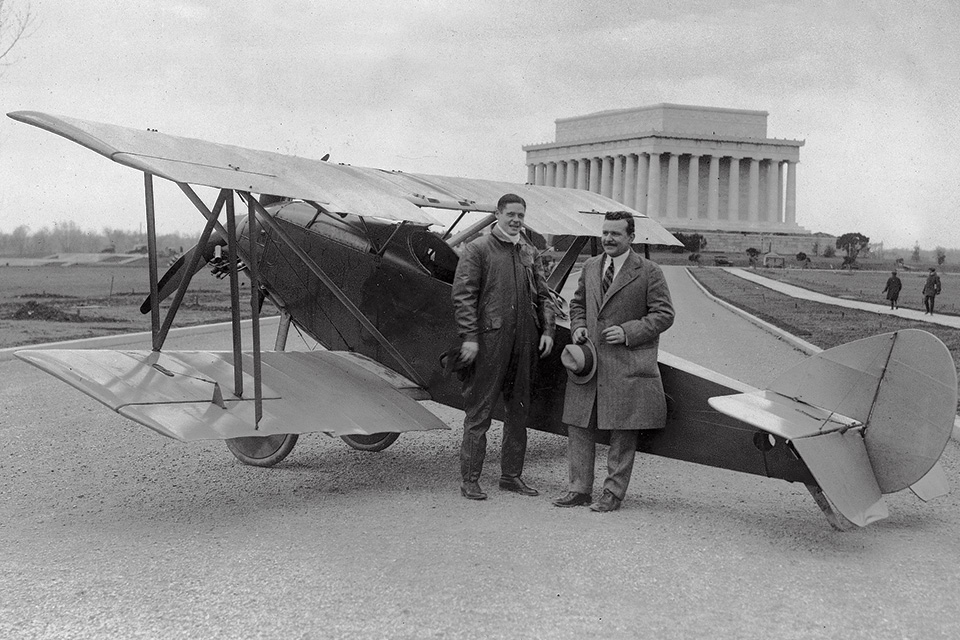
\includegraphics[scale=0.30]{obr2.jpg}
\caption{Lawrence Sperry (naľavo)}
\label{f:obr2}
\end{figure*}

\subsection{Autopilot v lietadlách} \label{ina:nejaka}
V letectve sa často stretávame s pomenovaním AFCS.\footnote{Automatic Flight Control Systems - automatické systémy riadenia letu}Tieto systémy sú univerzálne používané v komerčnom letectve. Rozsiahle uplatnenie nachádzajú aj vo vojenskom a všeobecnom letectve, ale koncepcia voľného letu, v rámci ktorej bude v budúcnosti prebiehať plne automatický let, je v podstate zameraná na zníženie preťaženia dýchacích ciest, čo je situácia, ktorá ovplyvňuje najmä komerčné letectvo. Hoci lietadlá všeobecného letectva wm musia tiež pracovať v prostredí voľného letu, väčšina týchto lietadiel má buď iba manuálne riadiace systémy, alebo je inštalácia AFCS len základná. 

Hlavným účelom použitia AFCS je do určitej miery automatizovať lietanie lietadla, aby sa znížila pracovná záťaž pilotov (zvyčajne v určitej kritickej fáze letu), aby sa zachovala bezpečnosť letu. Čoraz častejšie sa AFCS používajú aj na zlepšenie základných letových vlastností lietadla (napr. na zabezpečenie dynamickej stability, aj keď bolo lietadlo navrhnuté ako staticky nestabilné), alebo na overenie základných výkonov lietadla v niektorých atmosférických podmienkach. Na dosiahnutie plne automatického letu bude potrebné, aby sa dosiahlo niekoľko dôležitých technologických a operačných systémových vývojov, ale vždy, keď sa to podarí, výsledný plne automatický systém bude fungovať prostredníctvom už vyvinutého AFCS. 

\begin{figure*}[tbh]
\centering
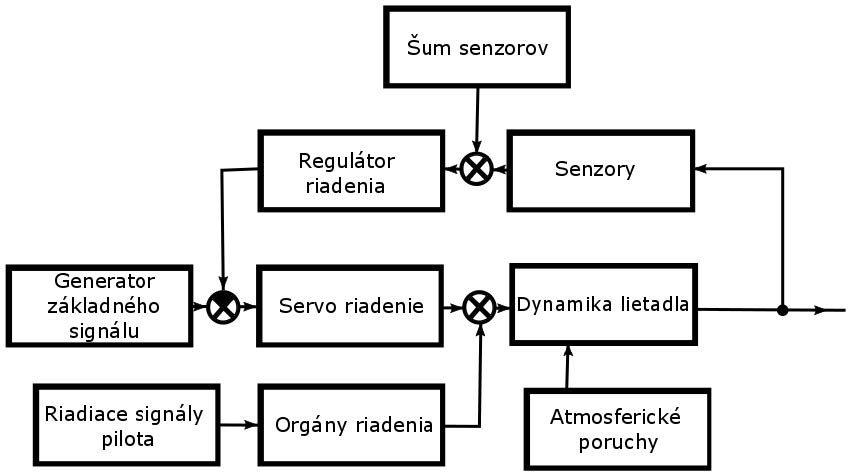
\includegraphics[scale=0.9]{obr1.jpg}
\caption{Funkčná schéma autopilota}
\label{f:obr1}
\end{figure*}

\section{Chyby autopilota} \label{chyby}

Základným problémom je teda\ldots{} Najprv sa pozrieme na nejaké vysvetlenie (časť~\ref{ina:nejake}), a potom na ešte nejaké (časť~\ref{ina:nejake}).\footnote{Niekedy môžete potrebovať aj poznámku pod čiarou.}

Môže sa zdať, že problém vlastne nejestvuje\cite{Coplien:MPD}, ale bolo dokázané, že to tak nie je~\cite{Czarnecki:Staged, Czarnecki:Progress}. Napriek tomu, aj dnes na webe narazíme na všelijaké pochybné názory\cite{PLP-Framework}. Dôležité veci možno \emph{zdôrazniť kurzívou}.


\subsection{Nejaké vysvetlenie} \label{ina:nejake}

%Niekedy treba uviesť zoznam:

%\begin{itemize}
%\item jedna vec
%\item druhá vec
	%\begin{itemize}
	%\item x
	%\item y
	%\end{itemize}
%\end{itemize}

%Ten istý zoznam, len číslovaný:

%\begin{enumerate}
%\item jedna vec
%\item druhá vec
%	\begin{enumerate}
%	\item x
%	\item y
%	\end{enumerate}
%\end{enumerate}


%\subsection{Ešte nejaké vysvetlenie} \label{ina:este}

%\paragraph{Veľmi dôležitá poznámka.}
%Niekedy je potrebné nadpisom označiť odsek. Text pokračuje hneď za nadpisom.



\section{Dôležitá časť} \label{dolezita}




\section{Ešte dôležitejšia časť} \label{dolezitejsia}




\section{Záver} \label{zaver} 



%\acknowledgement{Ak niekomu chcete poďakovať\ldots}


\bibliography{literatura}
\bibliographystyle{plain} 
\end{document}